\documentclass[12pt]{article}

\usepackage{import}
\usepackage{customPackage}

\pagestyle{fancy}
\fancyhead{}
\fancyfoot[C]{\thepage\ of \pageref{LastPage}}
\fancyfoot[L]{\textcolor{red}{Version préliminaire du 27/07/2023}}
\fancyfoot[R]{}

%\bibliography{biblioPHD}
\addbibresource{biblioPHD.bib}

\title{Search for compact binary coalescence\\ using a single gravitational waves detector\\ with the MBTA data analysis pipeline}
\author{Vincent Juste (IPHC Strasbourg)}
\date{May 2023}


\begin{document}
\dosecttoc

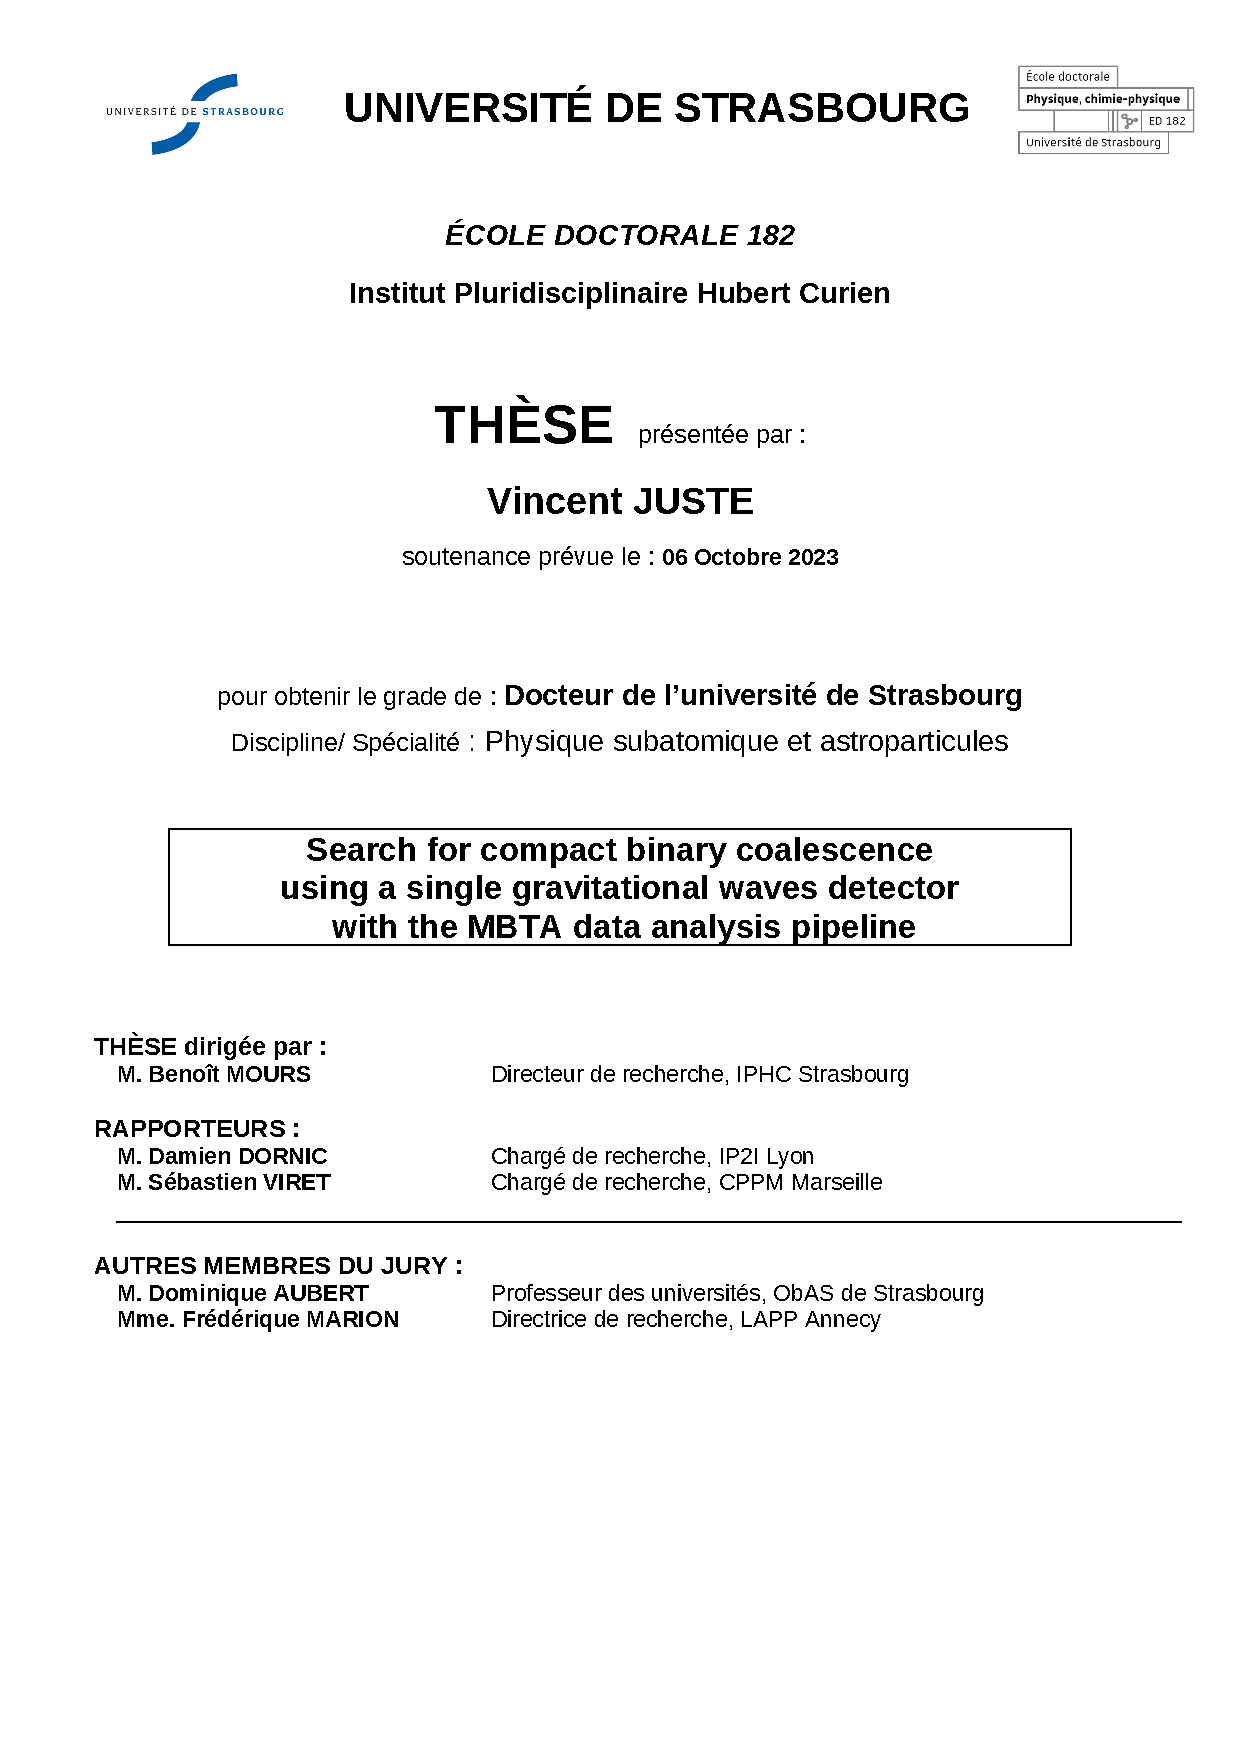
\includepdf[pages=1]{1er_4eme_couverture-ED182.pdf}

%\maketitle
\tableofcontents


\clearpage
\newpage
\section{Overview}
%\markright{}
%\addcontentsline{toc}{section}{Overview}
\label{section:overview}
\secttoc
\import{sectionOverview/}{sectionOverview.tex}




\clearpage
\newpage
\section{Ondes gravitationnelles}
\label{section:intro_gw}
\secttoc
\import{sectionGW/}{sectionGW.tex}






%%%%%%%%%%%%%%%%%%
%%%%%%%%%%%%%%%%%%
\clearpage
\newpage
\section{Détection des ondes gravitationelles}
\label{section:detection}
\secttoc
\import{sectionDetection/}{sectionDetection.tex}





%%%%%%%%%%%%%%%%%%
%%%%%%%%%%%%%%%%%%
\clearpage
\newpage
\section{Searching for CBC with MBTA}
\label{section:mbta}
\secttoc
\import{sectionMBTA/}{sectionMBTA.tex}






%%%%%%%%%%%%%%%%%%
%%%%%%%%%%%%%%%%%%
\clearpage
\newpage
\section{Selecting single detector triggers}
\label{section:selection}
\secttoc
\import{sectionSelection/}{sectionSelection.tex}




%%%%%%%%%%
%%%%%%%%%%
\clearpage
\newpage
\section{Assessing the significance of single detector triggers}
\label{section:far}
\secttoc
\import{sectionFAR/}{sectionFAR.tex}






%%%%%%%%%%%%%%%%%%
%%%%%%%%%%%%%%%%%%
\clearpage
\newpage
\section{Improving the rwSNR}
\label{section:rwSnr}
\secttoc
\import{sectionImprovement/}{sectionImprovement.tex}



%%%%%%%%%%%%%%%%%%
%%%%%%%%%%%%%%%%%%
\clearpage
\newpage
\section{Trigger rate and PSD fluctuations}
\label{section:bad_triggers}
\secttoc
\import{sectionBadTriggers/}{sectionBadTriggers.tex}


%%%%%%%%%%
%%%%%%%%%%
\clearpage
\newpage
\section{Single detector search during the begining of O4}
\label{section:O4}
\secttoc
\import{sectionO4/}{sectionO4.tex}



%%%%%%%%%%
%%%%%%%%%%
\clearpage
\newpage
\section{Conclusion}
\label{section:conclusion}
\secttoc
\import{sectionConclusion/}{sectionConclusion.tex}




%%%%%%%%%%
%%%%%%%%%%
\clearpage
\newpage

%\nocite{*}
\printbibliography

\includepdf[pages=2]{1er_4eme_couverture-ED182.pdf}

\end{document}
